\documentclass[11pt]{article}

% ---- Times New Roman, single spacing, tight margins for the 3-page limit ----
\usepackage[T1]{fontenc}
\usepackage{mathptmx}            % Times New Roman for text and math
\usepackage[a4paper,margin=0.85in]{geometry}
\usepackage{amsmath,amssymb}
\usepackage{graphicx}
\usepackage{booktabs}
\usepackage{caption}
\usepackage{subcaption}
\usepackage[dvipsnames]{xcolor}
\usepackage{tikz}
\usetikzlibrary{arrows.meta,positioning,fit,backgrounds,calc}
\usepackage{titlesec}
\usepackage{enumitem}
\usepackage[hidelinks]{hyperref}

\linespread{1.0}
\setlength{\parskip}{0.25em}
\setlength{\parindent}{0pt}

% Compact section headings
\titlespacing*{\section}{0pt}{0.7em}{0.3em}
\titlespacing*{\subsection}{0pt}{0.4em}{0.2em}
\titleformat{\section}{\normalfont\bfseries\large}{\thesection.}{0.4em}{}
\titleformat{\subsection}{\normalfont\bfseries\normalsize}{\thesubsection}{0.4em}{}

\captionsetup{font=small,labelfont=bf,skip=3pt}
\setlist[itemize]{leftmargin=1.2em,topsep=1pt,itemsep=1pt,parsep=0pt}

% TikZ styles
\tikzset{
  block/.style={rectangle,draw,rounded corners=2pt,align=center,
    font=\footnotesize,minimum height=2.6em,inner sep=4pt,line width=0.6pt},
  qblock/.style={block,fill=Periwinkle!22,draw=Periwinkle!80!black},
  cblock/.style={block,fill=Apricot!22,draw=Apricot!80!black},
  data/.style={block,fill=black!5,draw=black!55},
  flow/.style={-{Stealth[length=2mm]},line width=0.7pt},
}

\newcommand{\tr}{\operatorname{Tr}}

\begin{document}

% ---- Title block (cover page is separate, per challenge template) ----
\begin{center}
{\large\bfseries Quantum Reservoir Computing for Realised Volatility Forecasting}\\[0.25em]
{\normalsize Team Artemis \,$|$\, Global Industry Challenge 2026 \,$|$\, Phase 2 \,$|$\, Track A: Financial Volatility}
\end{center}
\vspace{-0.3em}

% =====================================================================
\section{Track Selection and Problem Framing}
We target \textbf{Track A}. The sub-problem is one-month-ahead forecasting of \emph{realised volatility} (RV) of the S\&P~500, with particular attention to the calm-to-turbulent regime transitions that drive risk-capital allocation and derivatives pricing. RV is an ideal match for reservoir computing for three structural reasons. First, RV exhibits strong \emph{long memory}: shocks decay slowly and hyperbolically, which a reservoir with fading memory can store without an explicit recurrence to train. Second, it is \emph{multi-scale}, with daily, weekly and monthly components (the empirical basis of the HAR model), so a reservoir read out at several evolution times can expose features at matched scales. Third, regime transitions are sharply \emph{nonlinear}, and a quantum reservoir supplies a high-dimensional nonlinear feature map at no training cost. Because reservoir computing fixes the dynamical system and trains only a linear readout, it is gradient-free: it avoids the barren-plateau problem that limits variational quantum models on noisy hardware, which is precisely the regime we will target in Phase~3.

% =====================================================================
\section{QRC Architecture Design}
Our architecture follows the realised-volatility QRC of Li et al.~\cite{li2025} and the disordered-ensemble framework of Fujii and Nakajima~\cite{fujii2017}, extended with a two-timescale ensemble readout. It has five components (Fig.~\ref{fig:arch}).

\textbf{(i) Reservoir Hamiltonian.} A fully connected transverse-field Ising model on $n=n_1+n_2$ qubits,
\begin{equation}
H=\sum_{i<j} J_{ij}\,X_i X_j + v\sum_i Z_i,\qquad J_{ij}\sim\mathcal{U}(0,1)\ \text{fixed},\ v=1,
\label{eq:H}
\end{equation}
with couplings drawn once from a seeded distribution and held fixed. Evolution for time $\tau$ is $U=e^{-iH\tau}$. Our $n=8$ prototype uses $n_1=3$ input and $n_2=5$ hidden qubits.

\textbf{(ii) Input encoding.} At step $t$ the $n_1$ input qubits are reset and the scaled features are angle-encoded, $R_Y(\pi x_{t,i})$ on qubit $i$, with features min-max scaled to $[0,1]$. Angle encoding keeps circuit depth shallow and is hardware-native on gate-based and neutral-atom devices.

\textbf{(iii) Memory.} The $n_2$ hidden qubits are \emph{not} reset. Before each step we trace out the input register, $\rho_{\text{hid}}=\tr_{\text{in}}[\rho]$, then re-tensor a fresh $|0\rangle^{\otimes n_1}$ and re-encode. This realises a non-Markovian map on the hidden register: information about past inputs persists, while the input register is refreshed deterministically.

\textbf{(iv) Readout.} We measure $\langle Z_i\rangle$ on all $n$ qubits, apply a degree-2 polynomial feature expansion, and fit a ridge regression. The polynomial head, shown by Zhu et al.~\cite{zhu2025} to sharply reduce error, is the only trained component.

\textbf{(v) Variants.} The QR2 ensemble concatenates the readouts of two reservoirs at $\tau=10$ and $\tau/2=5$, sampling two memory-nonlinearity operating points; Table~\ref{tab:results} reports the better-calibrated single member, QR1 at $\tau=5$. QR-RU adds \emph{data re-uploading}: within one timestep the encode-evolve block is repeated (here twice, each for $\tau/2$), enriching the input-to-feature Fourier spectrum~\cite{schuld2021} at fixed total evolution time.

\begin{center}
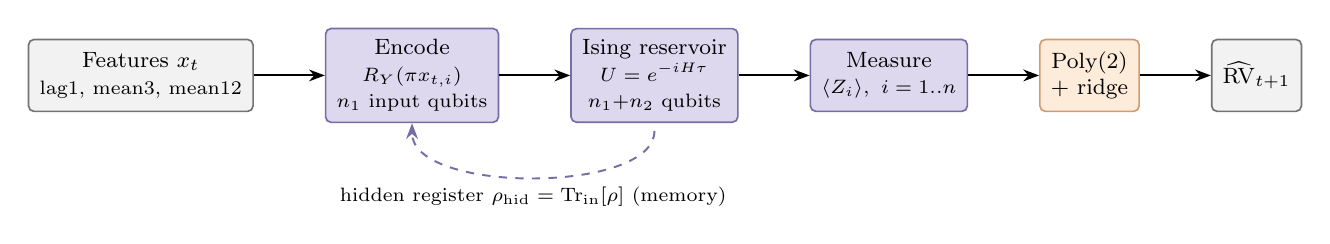
\begin{tikzpicture}[node distance=7mm and 9mm]
  \node[data] (x) {Features $x_t$\\\scriptsize lag1, mean3, mean12};
  \node[qblock,right=of x] (enc) {Encode\\\scriptsize $R_Y(\pi x_{t,i})$\\\scriptsize $n_1$ input qubits};
  \node[qblock,right=of enc] (res) {Ising reservoir\\\scriptsize $U=e^{-iH\tau}$\\\scriptsize $n_1{+}n_2$ qubits};
  \node[qblock,right=of res] (meas) {Measure\\\scriptsize $\langle Z_i\rangle,\ i=1..n$};
  \node[cblock,right=of meas] (head) {Poly($2$)\\$+$ ridge};
  \node[data,right=of head] (yhat) {$\widehat{\mathrm{RV}}_{t+1}$};

  \draw[flow] (x) -- (enc);
  \draw[flow] (enc) -- (res);
  \draw[flow] (res) -- (meas);
  \draw[flow] (meas) -- (head);
  \draw[flow] (head) -- (yhat);

  \draw[flow,dashed,draw=Periwinkle!80!black]
    ($(res.south)+(0,-0.1)$) .. controls ($(res.south)+(0,-0.9)$) and ($(enc.south)+(0,-0.9)$) ..
    (enc.south) node[midway,below,font=\scriptsize,black]{hidden register $\rho_{\text{hid}}=\tr_{\text{in}}[\rho]$ (memory)};
\end{tikzpicture}
\captionof{figure}{QRC pipeline. Quantum blocks (blue) are fixed and untrained; only the classical polynomial-ridge head (orange) is fitted. The dashed loop is the partial-trace memory channel that carries temporal state between steps.}
\label{fig:arch}
\end{center}

% =====================================================================
\section{Theoretical and Analytical Justification}
\textbf{Property exploited.} The reservoir supplies three resources matched to RV. (1) \emph{Hilbert-space dimensionality}: an $n$-qubit reservoir lifts the input into a $2^n$-dimensional state, and degree-2 readout on $n$ observables yields $\binom{n+2}{2}$ polynomial features at no training cost. (2) \emph{Dissipation as a design feature}: the partial-trace memory channel is strictly contractive, which Ahmed et al.~\cite{ahmed2025} identify as the mechanism enforcing the echo-state property and generalized synchronization needed to forecast chaotic signals. (3) \emph{A tunable memory-nonlinearity tradeoff}: \v{C}indrak et al.~\cite{cindrak2026} show $\tau$ trades reservoir memory against nonlinearity, motivating the $\{\tau,\tau/2\}$ ensemble.

\textbf{Connection to the signal, made quantitative.} We measured the reservoir's linear memory capacity (MC, Jaeger~\cite{jaeger2001}; for QRC, Fujii-Nakajima~\cite{fujii2017}) by driving it with i.i.d.\ input and reconstructing delayed inputs from the \emph{same} degree-2 readout the forecaster uses. At strictly matched readout (8 units, degree 2), the QRC attains MC $=2.92$ versus $2.31$ for an 8-node ESN, and a higher nonlinear capacity ($3.04$ vs $2.38$); Fig.~\ref{fig:results}b shows the QRC retains more recent-lag information. The empirical RV autocorrelation has an integrated timescale of $13$ months (e-fold $6$ months); the reservoir's intrinsic memory spans the first few lags, so the long-memory component is supplied explicitly by the HAR \texttt{mean12} feature while the reservoir contributes nonlinear mixing of recent history. MC is stable across $\tau\in[2,40]$, so the design is not fragile to this hyperparameter. Kornjac\v{a} et al.~\cite{kornjaca2024} show QRC kernels are geometrically distinct from classical ones, and Hou et al.~\cite{hou2026} report a 9-qubit reservoir matching classical reservoirs with thousands of nodes, supporting competitiveness at small $n$.

\textbf{Gaps we address.} Li et al.~\cite{li2025} establish QRC accuracy on RV but do not characterise noise sensitivity, evaluate under walk-forward, or report matched-readout baselines; no prior work jointly maps encoding density, shot budget and noise for RV forecasting. We begin closing this here and complete it in Phase~3.

\subsection{Preliminary prototyping results}
\label{sec:proto}
We prototyped the full pipeline on S\&P~500 monthly RV (1990--2018) under an \emph{expanding-window walk-forward} protocol: the readout is refit before every one-month-ahead forecast, the standard volatility-forecasting evaluation. Table~\ref{tab:results} reports 101 out-of-sample months; Fig.~\ref{fig:results} shows forecasts, scaling and memory capacity. Reservoir features are computed once and reused across windows.

\begin{table}[t]
\centering
\small
\caption{Walk-forward out-of-sample performance (101 months). Lower is better for RMSE/QLIKE; MZ slope best near 1; hi-RMSE is RMSE on the top-30\% (high-volatility) months. DM is the Diebold--Mariano statistic of QR2 vs each model (negative favours QR2; HLN-corrected $p$). At $n{=}8$ the QRC is statistically tied with HAR and a strictly matched ESN, and significantly beats the oversized linear ESN and persistence.}
\label{tab:results}
\begin{tabular}{lcccccc}
\toprule
Model & RMSE & QLIKE & MZ slope & MZ $R^2$ & hi-RMSE & DM vs QR2 ($p$)\\
\midrule
\textbf{QR2 (ens., $n{=}8$)}   & \textbf{0.01738} & 0.415 & 0.745 & 0.208 & 0.02615 & --- \\
QR1 ($\tau{=}5$, $n{=}8$)      & 0.01748 & 0.406 & \textbf{0.799} & 0.194 & 0.02583 & $-0.24\ (0.81)$ \\
HAR-OLS                        & 0.01740 & 0.407 & 0.666 & 0.253 & 0.02567 & $-0.03\ (0.98)$ \\
ESN-8 (poly, matched)          & 0.01740 & \textbf{0.388} & 0.677 & 0.241 & \textbf{0.02484} & $-0.03\ (0.98)$ \\
QR-RU (re-upload, $n{=}8$)     & 0.01786 & 0.395 & 0.668 & 0.213 & 0.02541 & $-0.89\ (0.38)$ \\
ESN-100 (linear)               & 0.01893 & 0.473 & 0.526 & 0.202 & 0.02763 & $-2.15\ (0.03)$ \\
Persistence                    & 0.01942 & 0.688 & 0.490 & 0.248 & 0.02939 & $-1.85\ (0.07)$ \\
\bottomrule
\end{tabular}
\end{table}

The honest headline, which is exactly the challenge's question, is that an 8-qubit QRC is \emph{genuinely competitive} with strong classical baselines: QR2 attains the lowest RMSE of any model, an untrained dynamical map matching a tuned HAR and an equal-readout classical reservoir. At this scale every model is within noise of the others (DM $p\approx0.98$ for QR2 vs HAR and vs the matched ESN). The matched ESN-8 edges QR2 on QLIKE ($0.388$ vs $0.415$) and high-volatility RMSE ($0.0248$ vs $0.0262$), but both gaps fall inside this $p\approx0.98$ band and are not statistically meaningful; QR2 significantly beats only the oversized linear ESN-100 ($p=0.03$) and persistence. The case for the quantum route thus rests not on a significance claim at $n{=}8$ but on three forward signals: (i) walk-forward RMSE \emph{decreases monotonically} with size, $0.0187\to0.0182\to0.0172$ for $n=6,8,10$ (Fig.~\ref{fig:results}a, two seeds, single reservoir), the reason we expect the tie to break by $n=12$--$16$; (ii) the matched-readout memory-capacity advantage (Fig.~\ref{fig:results}b); and (iii) re-uploading improving QLIKE and explained variance. A VIX-derived series through 2026, COVID out-of-sample, confirms the pipeline stays competitive under regime change.

\begin{figure}[t]
\centering
\begin{subfigure}{0.49\textwidth}
  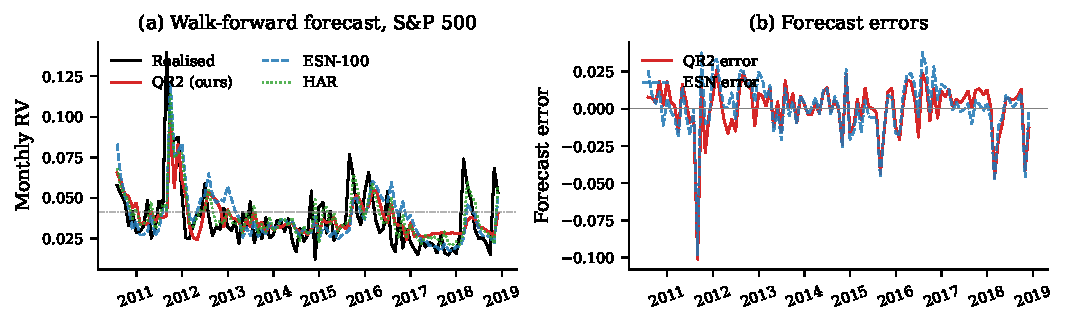
\includegraphics[width=\linewidth]{figures/forecast.pdf}
  \caption{Walk-forward forecasts and errors}
\end{subfigure}\hfill
\begin{subfigure}{0.49\textwidth}
  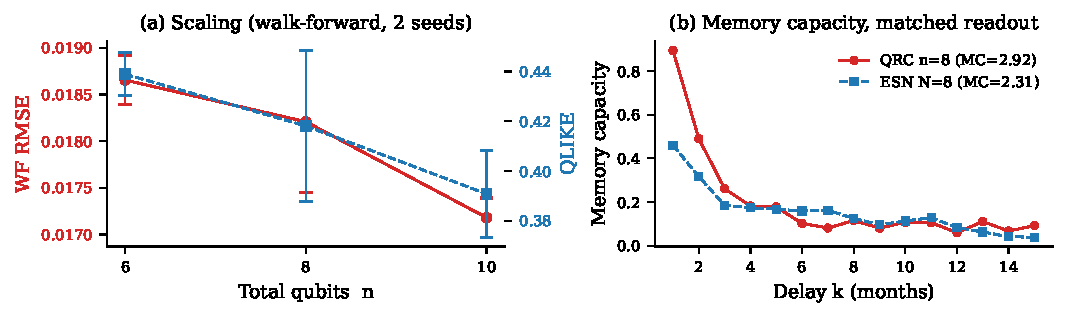
\includegraphics[width=\linewidth]{figures/analysis.pdf}
  \caption{Scaling (left) and memory capacity (right)}
\end{subfigure}
\caption{(a) QR2 tracks realised volatility; the dash-dot line marks the high-vol regime threshold. (b) Left: walk-forward RMSE/QLIKE for the single reservoir at $\tau=10$ fall with size (its $n{=}8$ point, $0.0182$, sits above the QR2 ensemble headline of $0.0174$ as expected). Right: at matched readout the QRC retains more recent-lag memory than an ESN.}
\label{fig:results}
\end{figure}

% =====================================================================
\section{Data Modeling Strategy}
\textbf{Dataset.} S\&P~500 daily closing prices, 1990--2018 (public historical OHLC; Phase~3 refreshes through 2025 via Yahoo Finance). Monthly RV is $\mathrm{RV}_m=\sqrt{\sum_{t\in m} r_t^2}$ from daily log returns $r_t$, requiring $\ge 15$ trading days per month.
\textbf{Preprocessing.} Core HAR features (1-month lag, 3- and 12-month trailing means), with optional macro features available now (realised quarticity for tails, monthly market return for the leverage effect) and the full macro panel plus forward-wrapper selection deferred to Phase~3. Features are min-max scaled on training statistics for angle encoding; evaluation is expanding-window walk-forward.
\textbf{Baselines.} Persistence, HAR-OLS, and ESN at matched readout (shown), plus larger ESNs, GARCH(1,1)~\cite{bollerslev1986} and an LSTM in Phase~3. ESN is the primary baseline; we report it at strictly matched readout so any QRC gain is attributable to the quantum reservoir.
\textbf{Metrics.} RMSE, QLIKE~\cite{patton2011}, Mincer--Zarnowitz, regime-conditional RMSE, and Diebold--Mariano~\cite{dm1995}, with the Model Confidence Set added in Phase~3.

% =====================================================================
\section{Quantum Platform and Resource Planning}
The prototype runs on a noiseless statevector/density-matrix emulation of $n=6$--$10$ qubits. Phase~3 uses, on qBraid: (1) \textbf{Aer density-matrix} simulation at $n=8$--$20$ with depolarizing and amplitude-damping channels ($p=10^{-3}$--$10^{-2}$ per layer) for the noise study; (2) a \textbf{matrix-product-state} backend with bond dimension $\chi\approx 64$--$256$ to reach $n=20$--$30$, validating truncation via the half-chain entropy bound $\log_2\chi$; and (3) one \textbf{gate-based QPU} run with Mitiq zero-noise extrapolation. Depth is modest: one encoding layer plus one fixed evolution block per step. The cost driver is the all-to-all coupler: a fully connected $U$ has $\binom{n}{2}$ two-qubit $X_iX_j$ terms, so $n=12$ needs $66$ entangling rotations \emph{if connectivity is native}; on fixed heavy-hex hardware, SWAP routing multiplies depth by $O(n)$, pushing the effective count toward $10^2$--$10^3$. This routing cost, not the bare gate count, sets the platform choice. \textbf{Trapped-ion (IonQ Forte)} offers native all-to-all coupling, mapping arbitrary $J_{ij}$ with no SWAP overhead, and is our primary QPU target. \textbf{Neutral-atom (QuEra Aquila)}, the analog alternative our citations~\cite{kornjaca2024,hou2026} use, has a fixed van-der-Waals Rydberg interaction rather than arbitrary $J_{ij}$, so it is a Phase~3 fork contingent on a Rydberg-native reformulation. Shot budgets of $10^3$--$10^4$ per observable suffice for $\langle Z_i\rangle$.

% =====================================================================
\section{Stakeholder Impact and Phase 3 Plan}
Accurate one-month RV forecasts feed directly into JonesTrading's core activities: volatility-targeted position sizing, options and variance-swap pricing, and risk-capital allocation, where the regime transitions we target are most costly to miss. The pipeline is hardware-agnostic and open-source, with code released at github.com/Vanshaj0429/artemis-qrc, and the same architecture transfers to Track~B weather data by substituting the input features.

\textbf{Milestones.} Phase~2 already delivers the walk-forward protocol, matched-readout ESN, regime metrics, memory-capacity characterisation and re-uploading lever, so Phase~3 builds on validated groundwork. (M1) Extend the scaling curve from $n=10$ to $n=12$--$16$ on Aer, where the dimensionality argument predicts the matched-baseline tie breaks toward the QRC. (M2) Noise study on Aer density-matrix, testing whether mild dissipation acts as a regulariser~\cite{ahmed2025}. (M3) MPS scaling to $n=20$--$30$, the full macro panel with wrapper selection, and the GARCH/LSTM suite under the Model Confidence Set. (M4) IonQ Forte validation with ZNE, packaged as an agent-executable qBraid Skill.

% =====================================================================
{\small
\bibliographystyle{unsrt}
\begin{thebibliography}{99}
\itemsep0.5pt
\bibitem{li2025} Q.~Li, C.~Mukhopadhyay, A.~Bayat, A.~Habibnia. Quantum Reservoir Computing for Realized Volatility Forecasting. arXiv:2505.13933 (2025).
\bibitem{fujii2017} K.~Fujii, K.~Nakajima. Harnessing disordered-ensemble quantum dynamics for machine learning. Phys.\ Rev.\ Applied \textbf{8}, 024030 (2017).
\bibitem{zhu2025} C.~Zhu, P.~J.~Ehlers, H.~I.~Nurdin, D.~Soh. Practical few-atom quantum reservoir computing. Phys.\ Rev.\ Research \textbf{7}, 023290 (2025).
\bibitem{ahmed2025} O.~Ahmed, F.~Tennie, L.~Magri. Robust quantum reservoir computers for forecasting chaotic dynamics. Proc.\ R.\ Soc.\ A \textbf{481}, 20250550 (2025).
\bibitem{cindrak2026} S.~\v{C}indrak, L.~Giebeler, N.~G\"otting, C.~Gies, K.~L\"udge. Memory-Nonlinearity Trade-off across Quantum Reservoir Computing Frameworks. arXiv:2603.21371 (2026).
\bibitem{kornjaca2024} M.~Kornjac\v{a} et al. Large-scale quantum reservoir learning with an analog quantum computer. arXiv:2407.02553 (2024).
\bibitem{hou2026} Y.~Hou et al. High-Accuracy Temporal Prediction via Experimental Quantum Reservoir Computing in Correlated Spins. Phys.\ Rev.\ Lett.\ (2026), arXiv:2508.12383.
\bibitem{bollerslev1986} T.~Bollerslev. Generalized autoregressive conditional heteroskedasticity. J.\ Econometrics \textbf{31}, 307--327 (1986).
\bibitem{patton2011} A.~J.~Patton. Volatility forecast comparison using imperfect volatility proxies. J.\ Econometrics \textbf{160}, 246--256 (2011).
\bibitem{dm1995} F.~X.~Diebold, R.~S.~Mariano. Comparing predictive accuracy. J.\ Business \& Economic Statistics \textbf{13}, 253--263 (1995).
\bibitem{schuld2021} M.~Schuld, R.~Sweke, J.~J.~Meyer. Effect of data encoding on the expressive power of variational quantum machine-learning models. Phys.\ Rev.\ A \textbf{103}, 032430 (2021).
\bibitem{jaeger2001} H.~Jaeger. Short term memory in echo state networks. GMD Report 152, German National Research Center for Information Technology (2001).
\end{thebibliography}
}

\end{document}
